\section{End Users}
\label{sec:enduser}
%In this sections the group of end users are discovered. 
Since we are using \scrum{} as our primary development practice we prefer to have a product owner~\cite[p.~115]{Larman04} who can speak on behalf of the end users.
As mentioned in \secref{subsec:choosingmethod} we do not have a product owner, which is why we facilitate the contact and communication with the end users ourselves.
In this section the end users for our \subsystem{} are defined and the people that we use as representatives are presented shortly -- we cannot speak with all potential end users because there are too many.


\begin{figure}%
%\begin{landscape}
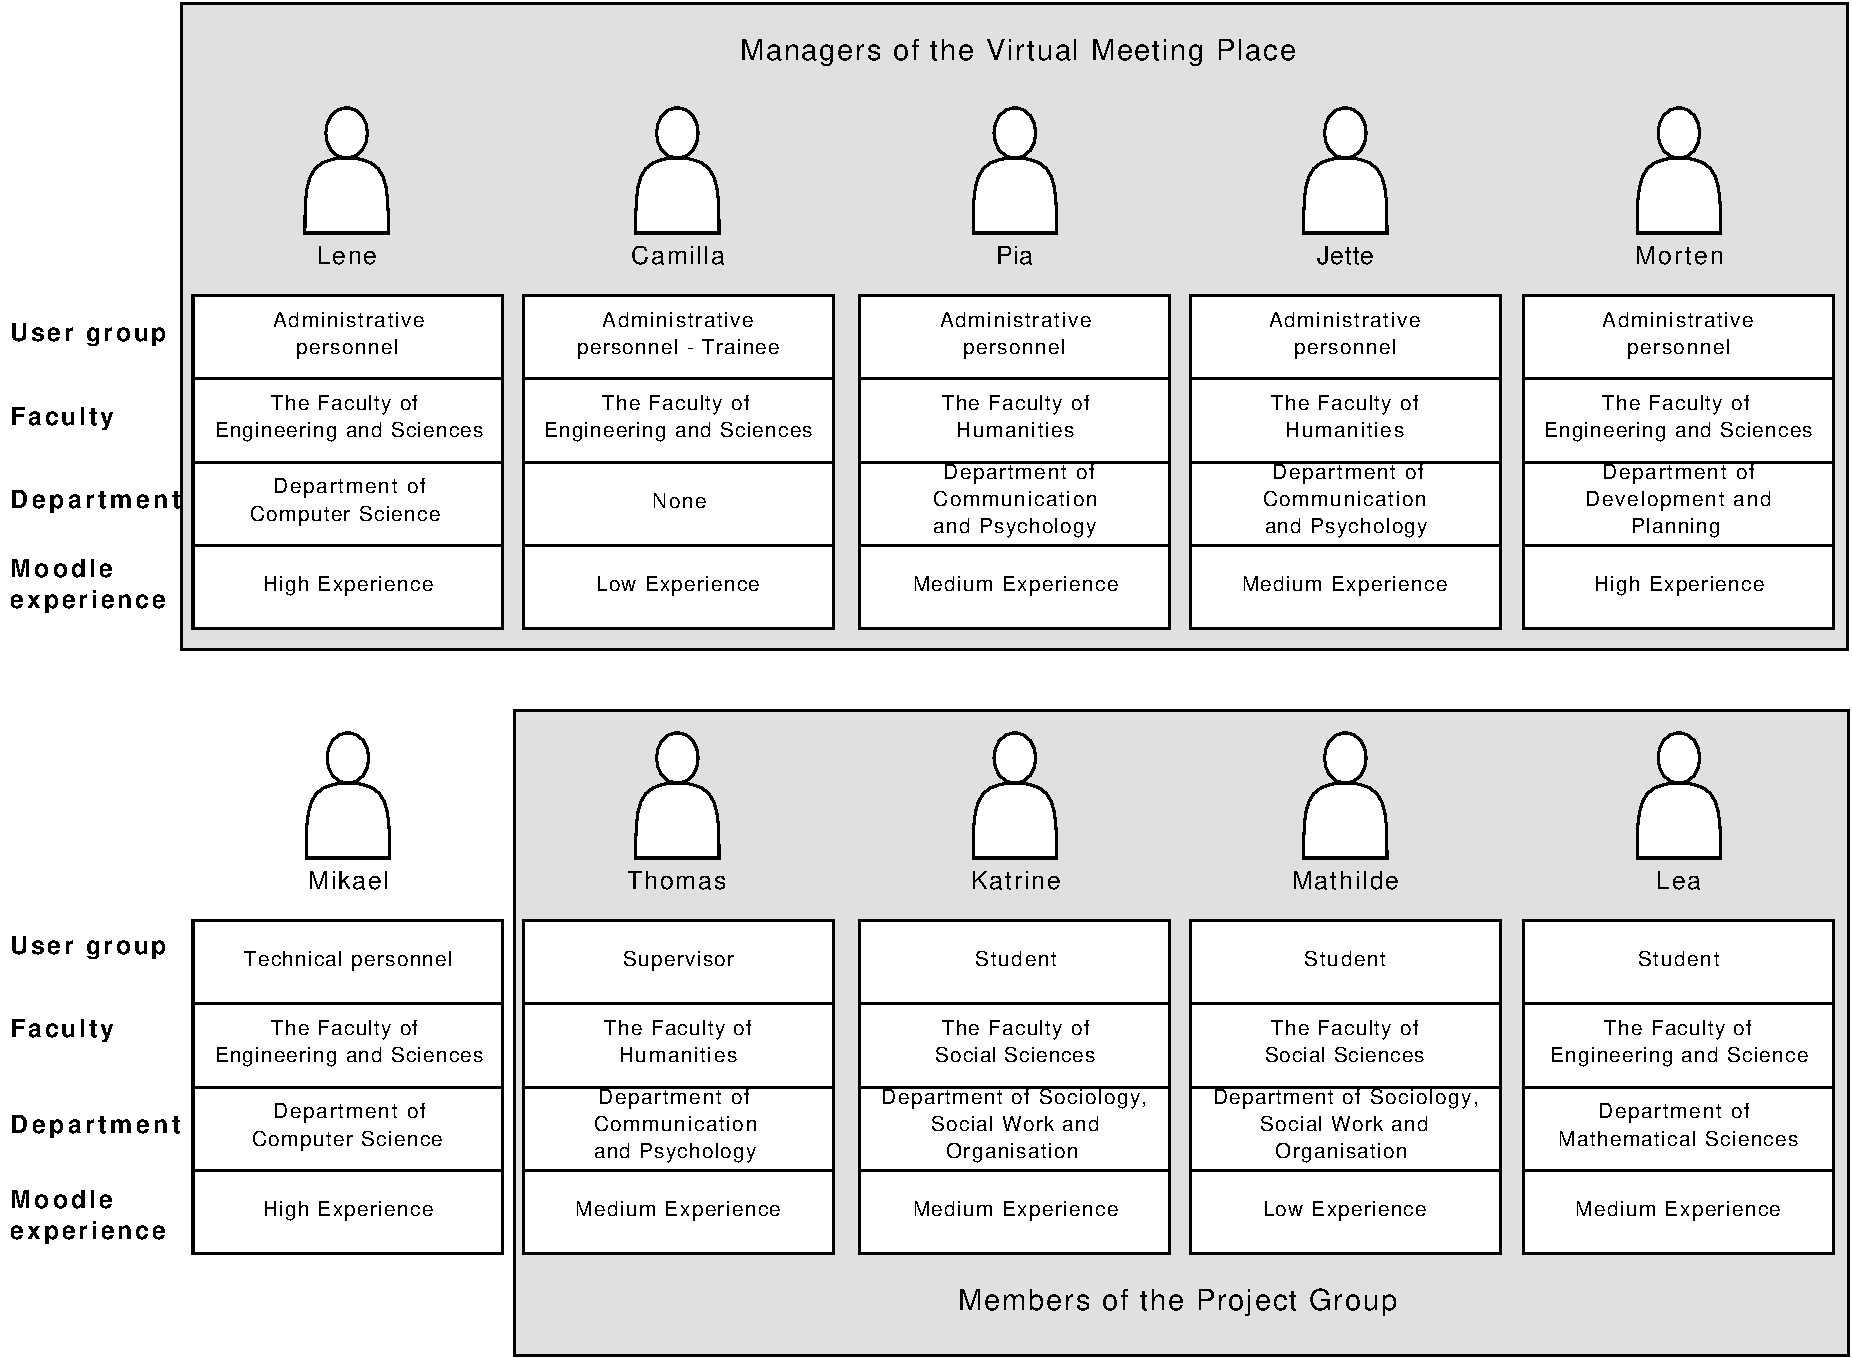
\includegraphics[angle=90,scale=0.45]{images/UserGroups2}%
\morscaption{An overview of our end users. 
The gray boxes contain the two categories of end users. 
The upper box contains the members of the project groups, the lower box is the managers of the project groups}%
\label{fig:usergroup}%
%\end{landscape}
\end{figure}


The end users of the entire system are very diverse.
In in our sub-system we are interested in two different categories of end users:
\begin{itemize}
	\item Users of the virtual group rooms.
	\item Managers of the project groups.
\end{itemize}
%The group of end users that are members of the project group may very well be the same as the managers of the virtual group room. 
The two categories of end users can overlap. 
When choosing representatives for our end users there are several properties that we want to cover. 
These properties are: Type, Faculty, Department, and LMS experience.
The type of an end user is one of four values: \admpers[c], technical personnel, supervisors, or students.
Moodle experience is a scale from low to high.
Faculty and department are the end user's actual department and faculty. %% Too much?
We want users of each type and within these types we consider Faculty and LMS experience as important factors to be diverse.
%In choosing different types of end users we focus on the following properties: 
We would like to have representatives that cover these two properties as much as possible.

%An overview of the different end users can be seen on 

The end users we are using come from Aalborg University.
The reason for this is three-fold.
Firstly we are implementing the Aalborg PBL model into Moodle, which means that Aalborg University comes as a natural choice to look for end users.
Secondly our project is being conducted at Aalborg University. 
Consequently it is easier for us to find people to participate from this university compared to other universities. 
Thirdly the system is to be used at Aalborg University.

In \secref{sub:endusersmembers} and \secref{sub:enduserstool} we explore the two different categories of end users. 
An overview of the chosen end users can be seen in \figref{fig:usergroup}.
The coverage of properties is illustrated in \figref{fig:memPG} and \figref{fig:adminPG}.


\subsection{Users of the Virtual Group Room}
\label{sub:endusersmembers}
As discussed in \chapref{chap:systemDef} our responsibility is to create the concept of a project group and virtual group room.
Also we want to create a tool to manage project groups.
%For the concept of project group a group of students will function as our target group.
Since we are working together with three other peer-groups we receive requests for functionality from them.
Our peer-groups have their own end users, both students and supervisors, where they get their requests from.

To obtain an understanding of the members of the project groups we consider two different approaches:  
\begin{itemize}
\item Regarding students as a part of our end users and make our own field studies.
\item Relying on the requests of our peer-groups and effectively use our peer-groups as end user representatives.
\end{itemize}
%Alternatively we can choose to rely on our peer-groups requests and effectively use our peer-groups as our target group.
We choose a compromise and rely on the requests of our peer-groups and cooperate in the field studies related to the entire system and the concept of project groups.
By doing so we receive feedback directly from end users, which helps us avoid misunderstandings.


The end users of the virtual group room are students and supervisors.
We want to have different kinds of student representatives -- in particular students from different faculties.
We have two students from The Faculty of Social Sciences and one from The Faculty of Engineering and Sciences.
These are respectively Katrine Holmgaard Dinitzen, Mathilde Gammelgaard, and Lea Gustafsson.
Regarding supervisors, we choose to have a single representative; Thomas Ryberg Vibjerg Hansen~\cite{thomas}, who is supervisor under The Faculty of Humanities.
In \figref{fig:memPG} end user representatives of the virtual group room can be seen along with their LMS experience and faculty.

\begin{figure}%
\center
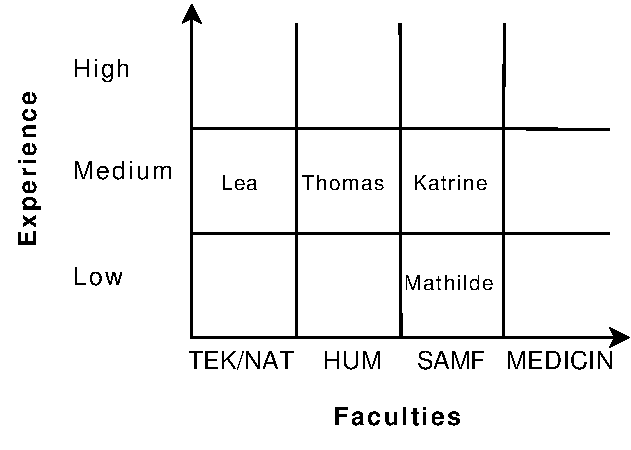
\includegraphics[scale=0.50]{images/MembersofpROJECTgROUJP}%
\morscaption{A graph showing how the end user representatives of the users of virtual group room are spread between faculties and how much experience they have with regard to LMSs}%
\label{fig:memPG}%
\end{figure}

%We focus on students since our peer-group \supervisorgroup{}

\subsection{Managers of Project Groups}
\label{sub:enduserstool}
We choose the \admpers{} as our end users because they have a good knowledge of project groups and the related management tasks.
From our own faculty we have the representatives Lene Winther Even~\cite{lene}, Camilla G\ae{}raa Larsen~\cite{camilla}, and Mikael M\o{}ller Hansen~\cite{mikael}.
Where Lene is a senior secretary, Camilla is an office trainee, and Mikael is an IT administrator.
We have been in contact with  Jette Due Nielsen~\cite{jette} and Pia Knudsen~\cite{piak} as our representatives from The Faculty of Social Sciences.
We have also been in contact with Morten Mathiasen Andersen~\cite{morten} from MPBL education and The Faculty of Engineering and Sciences.
\figref{fig:adminPG} shows these representatives along with their faculty and LMS experience.

\begin{figure}%
\center
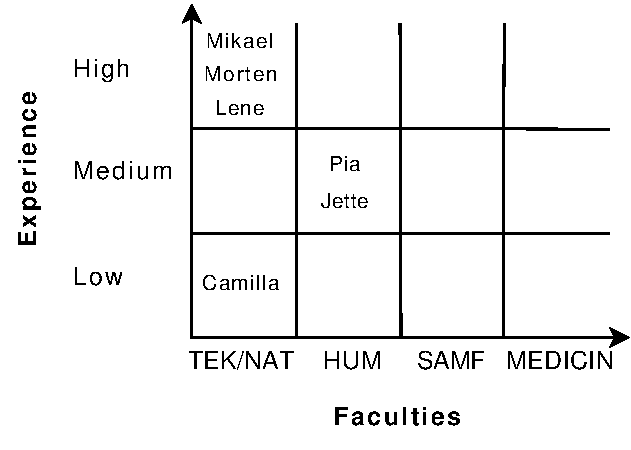
\includegraphics[scale=0.50]{images/administratorsOfPG}%
\morscaption{A graph showing how the end user representatives of the managers of project groups are spread between faculties and how much experience they have with regard to LMSs}%
\label{fig:adminPG}%
\end{figure}